\documentclass[11pt,a4paper]{article}
\usepackage[utf8]{inputenc}
\usepackage[T1]{fontenc}
\IfFileExists{lmodern.sty}{\usepackage{lmodern}}{}
\usepackage[margin=2.2cm]{geometry}
\usepackage{graphicx}
\usepackage{booktabs}
\usepackage{float}
\usepackage[hidelinks]{hyperref}
\setlength{\parskip}{0.5em}
\setlength{\parindent}{0pt}
\begin{document}
\begin{center}
{\LARGE EasyClassifier analysis report}\\[4pt]
{\large demo (Iris flowers)}\\[2pt]
09 October 2026 \quad$\cdot$\quad EasyClassifier 0.8.1
\end{center}
\section*{Summary}
The goal was to predict \emph{Species} from 4 other columns, using 149 rows. 7 classifiers were compared and \textbf{Neural Network (MLP)} was selected. Its honest final accuracy was \textbf{95.30\%} (guessing at random would give about 33\% with equally sized classes).
\section{Data and question}
File: demo (Iris flowers); 150 rows and 5 columns were loaded. Rows used in the analysis: 149.

\begin{table}[H]
\centering
\begin{tabular}{lrr}
\toprule
Class & Rows & Share\\
\midrule
setosa & 50 & 33.6\%\\
versicolor & 50 & 33.6\%\\
virginica & 49 & 32.9\%\\
\bottomrule
\end{tabular}
\caption{Classes of \emph{Species}.}
\end{table}
Predictor columns: sepal\_length, sepal\_width, petal\_length, petal\_width.

\begin{figure}[H]
\centering
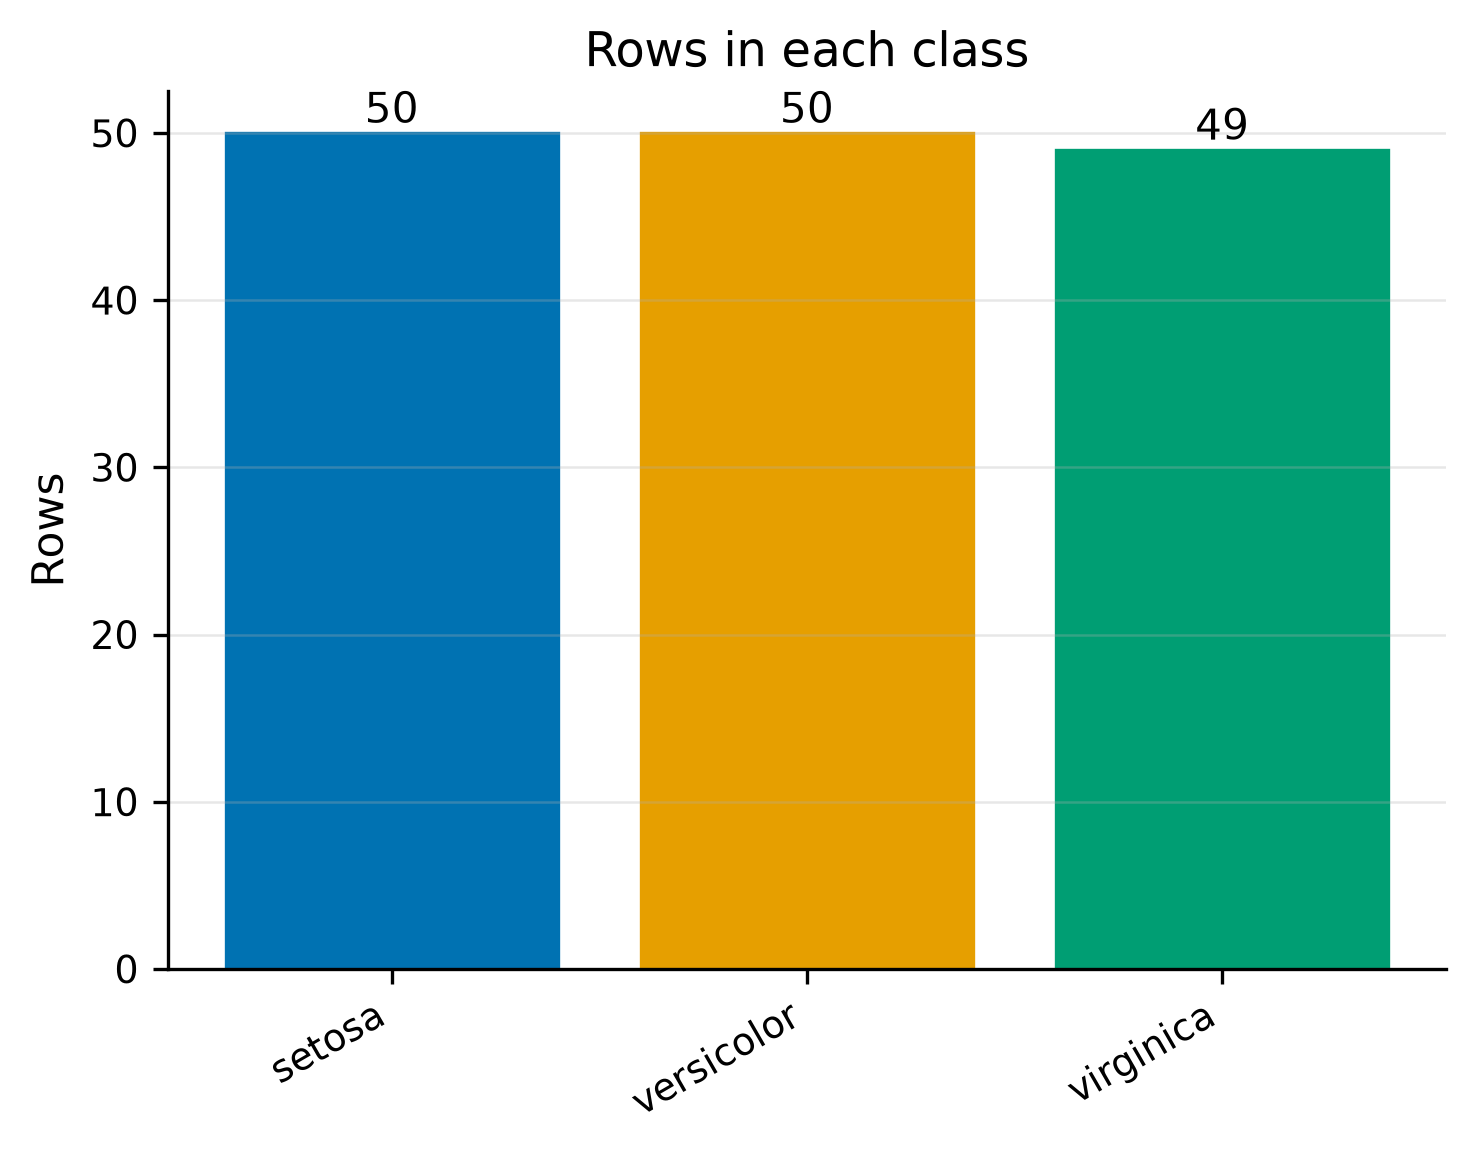
\includegraphics[width=0.62\textwidth]{figures/class_distribution.png}
\caption{Number of rows in each class. Very unequal classes make some measures (e.g.\ accuracy) look better than they are; balanced accuracy takes this into account.}
\end{figure}
\section{Methods (ready to adapt for your paper)}
The paragraph below describes exactly what was done. You may copy and adapt it for the methods section of a paper or thesis.

\begin{quote}
Classification was carried out with EasyClassifier version 0.8.1 \cite{easyclassifier}, which is built on scikit-learn \cite{sklearn}, NumPy \cite{numpy} and pandas \cite{pandas}. The dataset (demo (Iris flowers)) contained 150 rows and 5 columns. The outcome to predict was \emph{Species} with 3 classes. 1 duplicate row(s) were removed. The analysis used 149 rows and 4 predictor columns. Before modelling, numeric columns were standardised (mean 0, standard deviation 1) for Support Vector Machine (SVM), Logistic Regression and Neural Network (MLP), and scaled to the range 0--1 for KNN (Hassanat distance, k=5). All of these steps were learned from the training data only, separately within every validation split, so that no information from test data entered model training. The following classifiers were used with their default parameters, without hyperparameter tuning: Decision Tree \cite{breiman1984}, Random Forest \cite{breiman2001}, Support Vector Machine (SVM) \cite{cortes1995,platt1999}, Logistic Regression \cite{cox1958}, KNN (Hassanat distance, k=5) \cite{cover1967}, Naive Bayes \cite{hand2001} and Neural Network (MLP) \cite{rumelhart1986,kingma2015}. K-nearest neighbours used k = 5 and the Hassanat distance, applied in the standard form of the formula (all values non-negative) \cite{hassanat2022,hassanat2014}. Performance was estimated with 5-fold cross validation \cite{kohavi1995}. The classifier with the highest balanced accuracy was selected. To avoid optimistic bias from this selection, performance was estimated with nested 5-fold cross-validation, in which the complete comparison was repeated within each outer training fold and the winner was evaluated on the outer test fold \cite{varma2006,cawley2010}. The contribution of each predictor was estimated by permutation importance \cite{breiman2001}, i.e.\ the drop in balanced accuracy when that column's values were randomly shuffled, measured on the test part of each cross-validation fold. Classifiers were ranked by balanced accuracy \cite{brodersen2010}; the measures reported were Accuracy, Precision, Recall, F1 and ROC AUC \cite{fawcett2006}. Figures were drawn with Matplotlib \cite{matplotlib}, including ROC curves \cite{fawcett2006}.
\end{quote}
\section{Results}
\subsection*{Final result for Neural Network (MLP) (measured on nested cross-validation) -- report these numbers}
Support Vector Machine (SVM) chosen in 2/5 folds; Neural Network (MLP) chosen in 1/5 folds; Decision Tree chosen in 1/5 folds; Naive Bayes chosen in 1/5 folds.

\begin{table}[H]
\centering
\begin{tabular}{llp{0.57\textwidth}}
\toprule
Measure & Value & What it means\\
\midrule
Accuracy & 95.30\% & \parbox[t]{0.55\textwidth}{\small Accuracy is the share of predictions the model got right, out of all predictions.}\\[3pt]
Precision & 95.29\% & \parbox[t]{0.55\textwidth}{\small Precision measures how many of the items the model labeled positive are actually positive.}\\[3pt]
Recall & 95.29\% & \parbox[t]{0.55\textwidth}{\small Recall (sensitivity) measures how many of the real positive items the model successfully found.}\\[3pt]
F1 & 95.29\% & \parbox[t]{0.55\textwidth}{\small F1 is a single score that balances precision and recall. It is high only when both are high.}\\[3pt]
ROC AUC & 0.9633 & \parbox[t]{0.55\textwidth}{\small ROC AUC measures how well the model separates classes across all thresholds. 1.0 is perfect, 0.5 is random guessing.}\\[3pt]
\bottomrule
\end{tabular}
\end{table}
\subsection*{Comparison of classifiers}
These scores were used only to choose the best classifier. They are slightly optimistic, because the winner partly won by luck; report the final result above instead.

\begin{table}[H]
\centering
\small
\begin{tabular}{lrrrr}
\toprule
Classifier & Balanced accuracy & Accuracy & F1 & ROC AUC\\
\midrule
Neural Network (MLP) & 96.65\% & 96.64\% & 96.63\% & 0.9976\\
Logistic Regression & 96.64\% & 96.64\% & 96.63\% & 0.9978\\
Support Vector Machine (SVM) & 95.96\% & 95.97\% & 95.96\% & 0.9972\\
Decision Tree & 95.29\% & 95.30\% & 95.29\% & 0.9647\\
KNN (Hassanat distance, k=5) & 94.61\% & 94.63\% & 94.61\% & 0.9949\\
Random Forest & 94.60\% & 94.63\% & 94.61\% & 0.9935\\
Naive Bayes & 93.95\% & 93.96\% & 93.94\% & 0.9936\\
\bottomrule
\end{tabular}
\caption{Classifiers ranked by balanced accuracy.}
\end{table}
Neural Network (MLP) and Logistic Regression had the same balanced accuracy; Neural Network (MLP) was selected because it is listed first. They perform equally well on this data.

\begin{figure}[H]
\centering
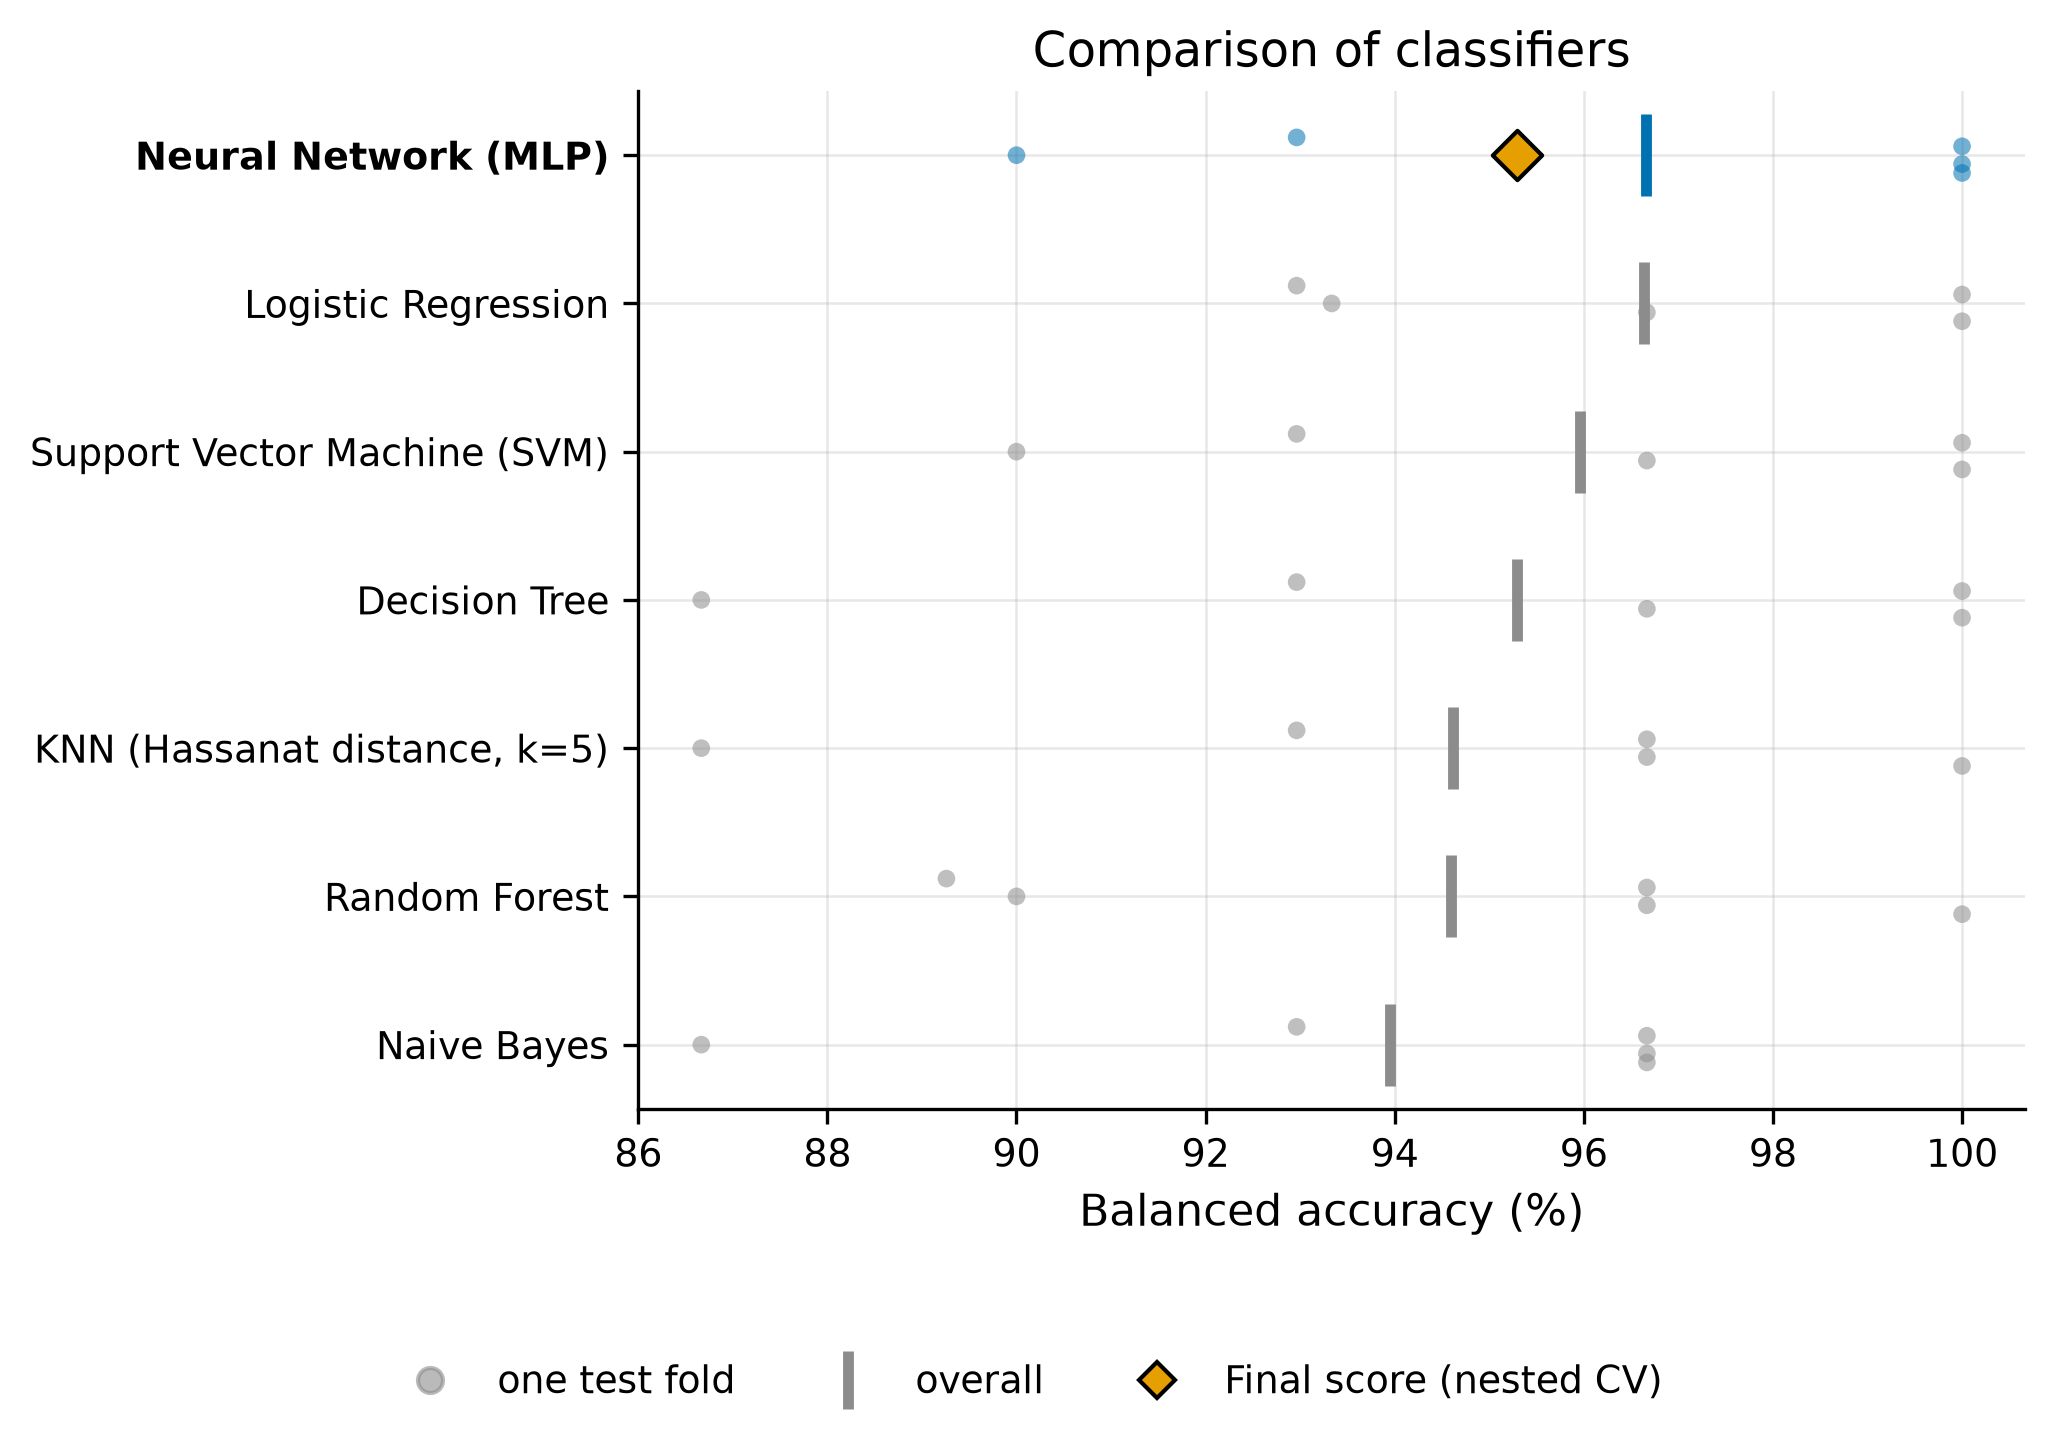
\includegraphics[width=0.8\textwidth]{figures/comparison.png}
\caption{Balanced accuracy of each classifier. Dots are the individual test folds, the vertical bar is the overall score. The wider the dots are spread, the less certain the ranking. The diamond, if shown, is the final score of the selected classifier on data not used to choose it.}
\end{figure}
\subsection*{Figures for Neural Network (MLP) (final result)}
\begin{figure}[H]
\centering
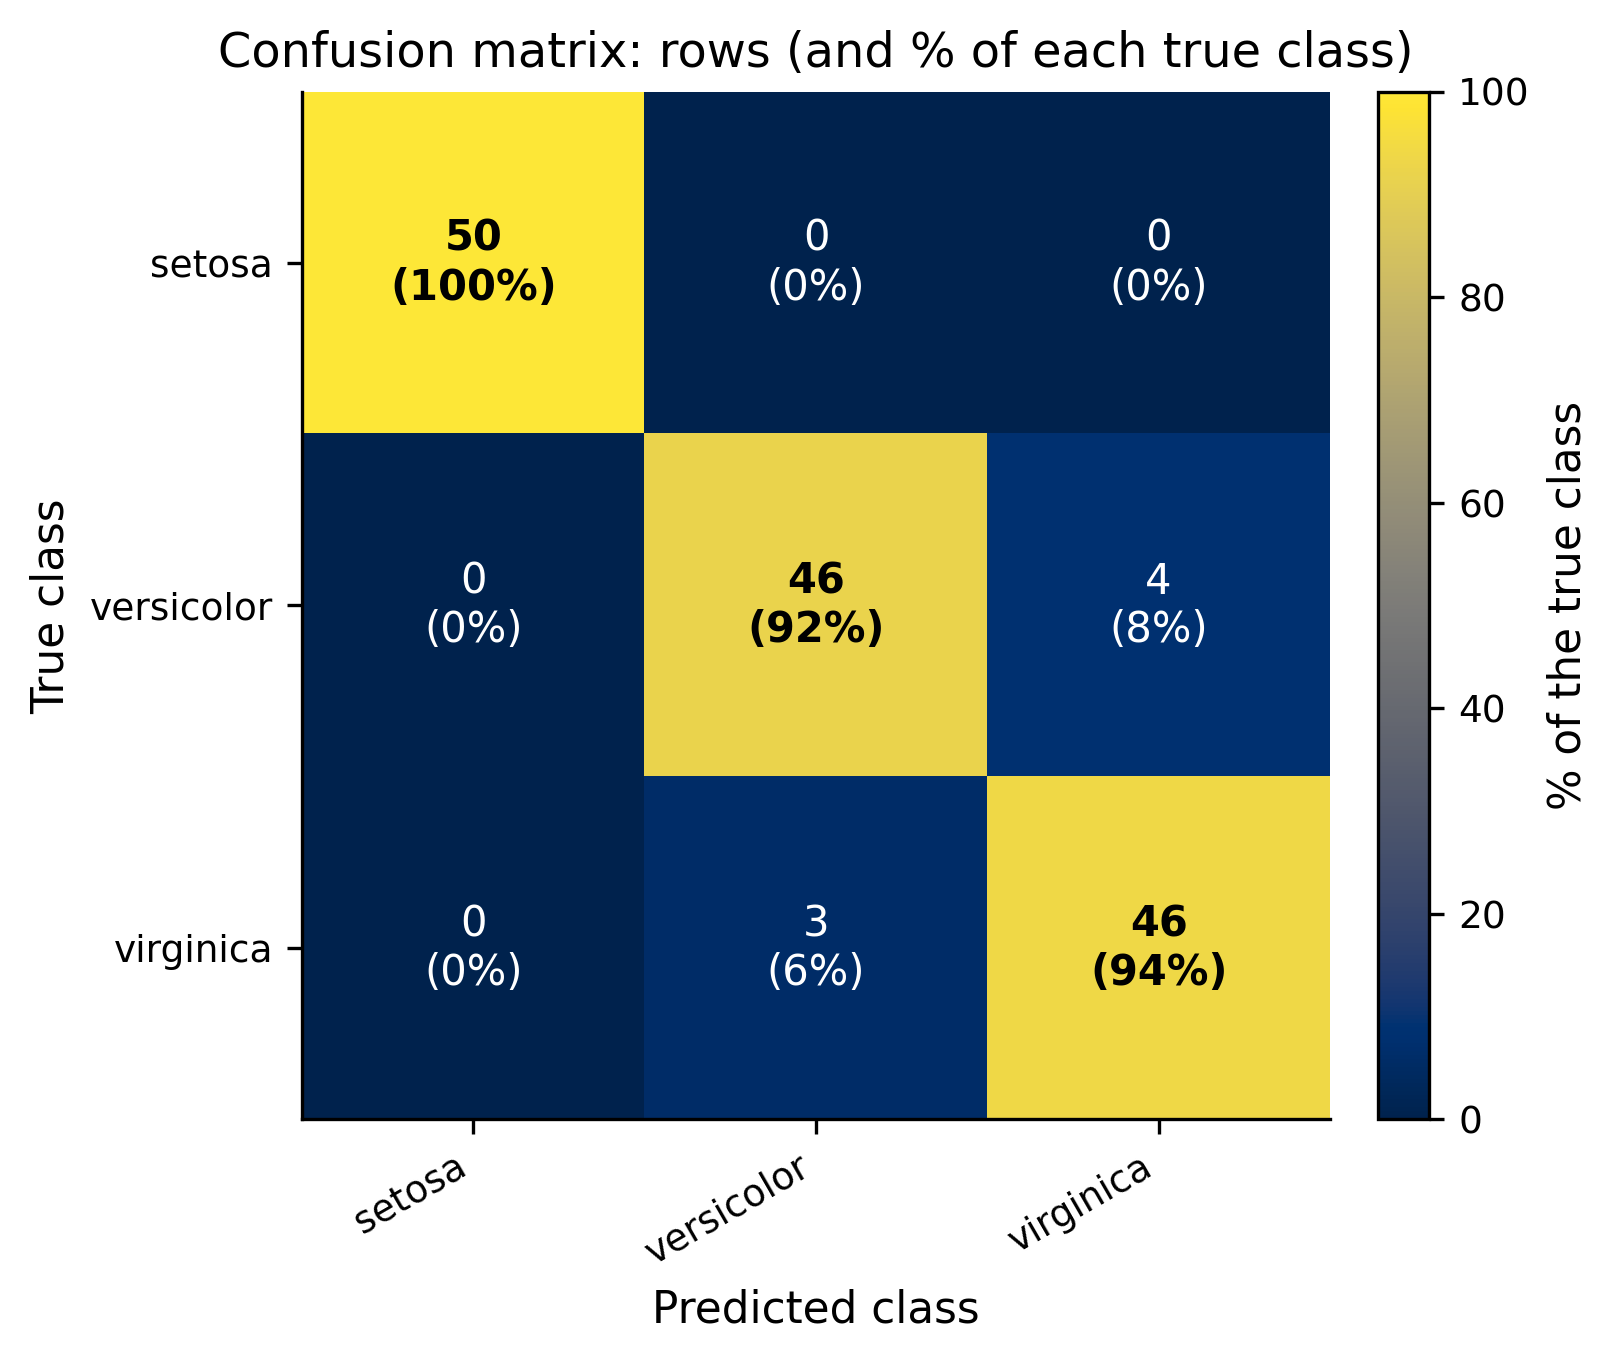
\includegraphics[width=0.62\textwidth]{figures/confusion_matrix.png}
\caption{Confusion matrix. Rows are the true classes, columns the predicted classes; each cell shows the number of rows and the percentage of that true class. The diagonal holds the correct predictions; off-diagonal cells show which classes are confused.}
\end{figure}
\begin{figure}[H]
\centering
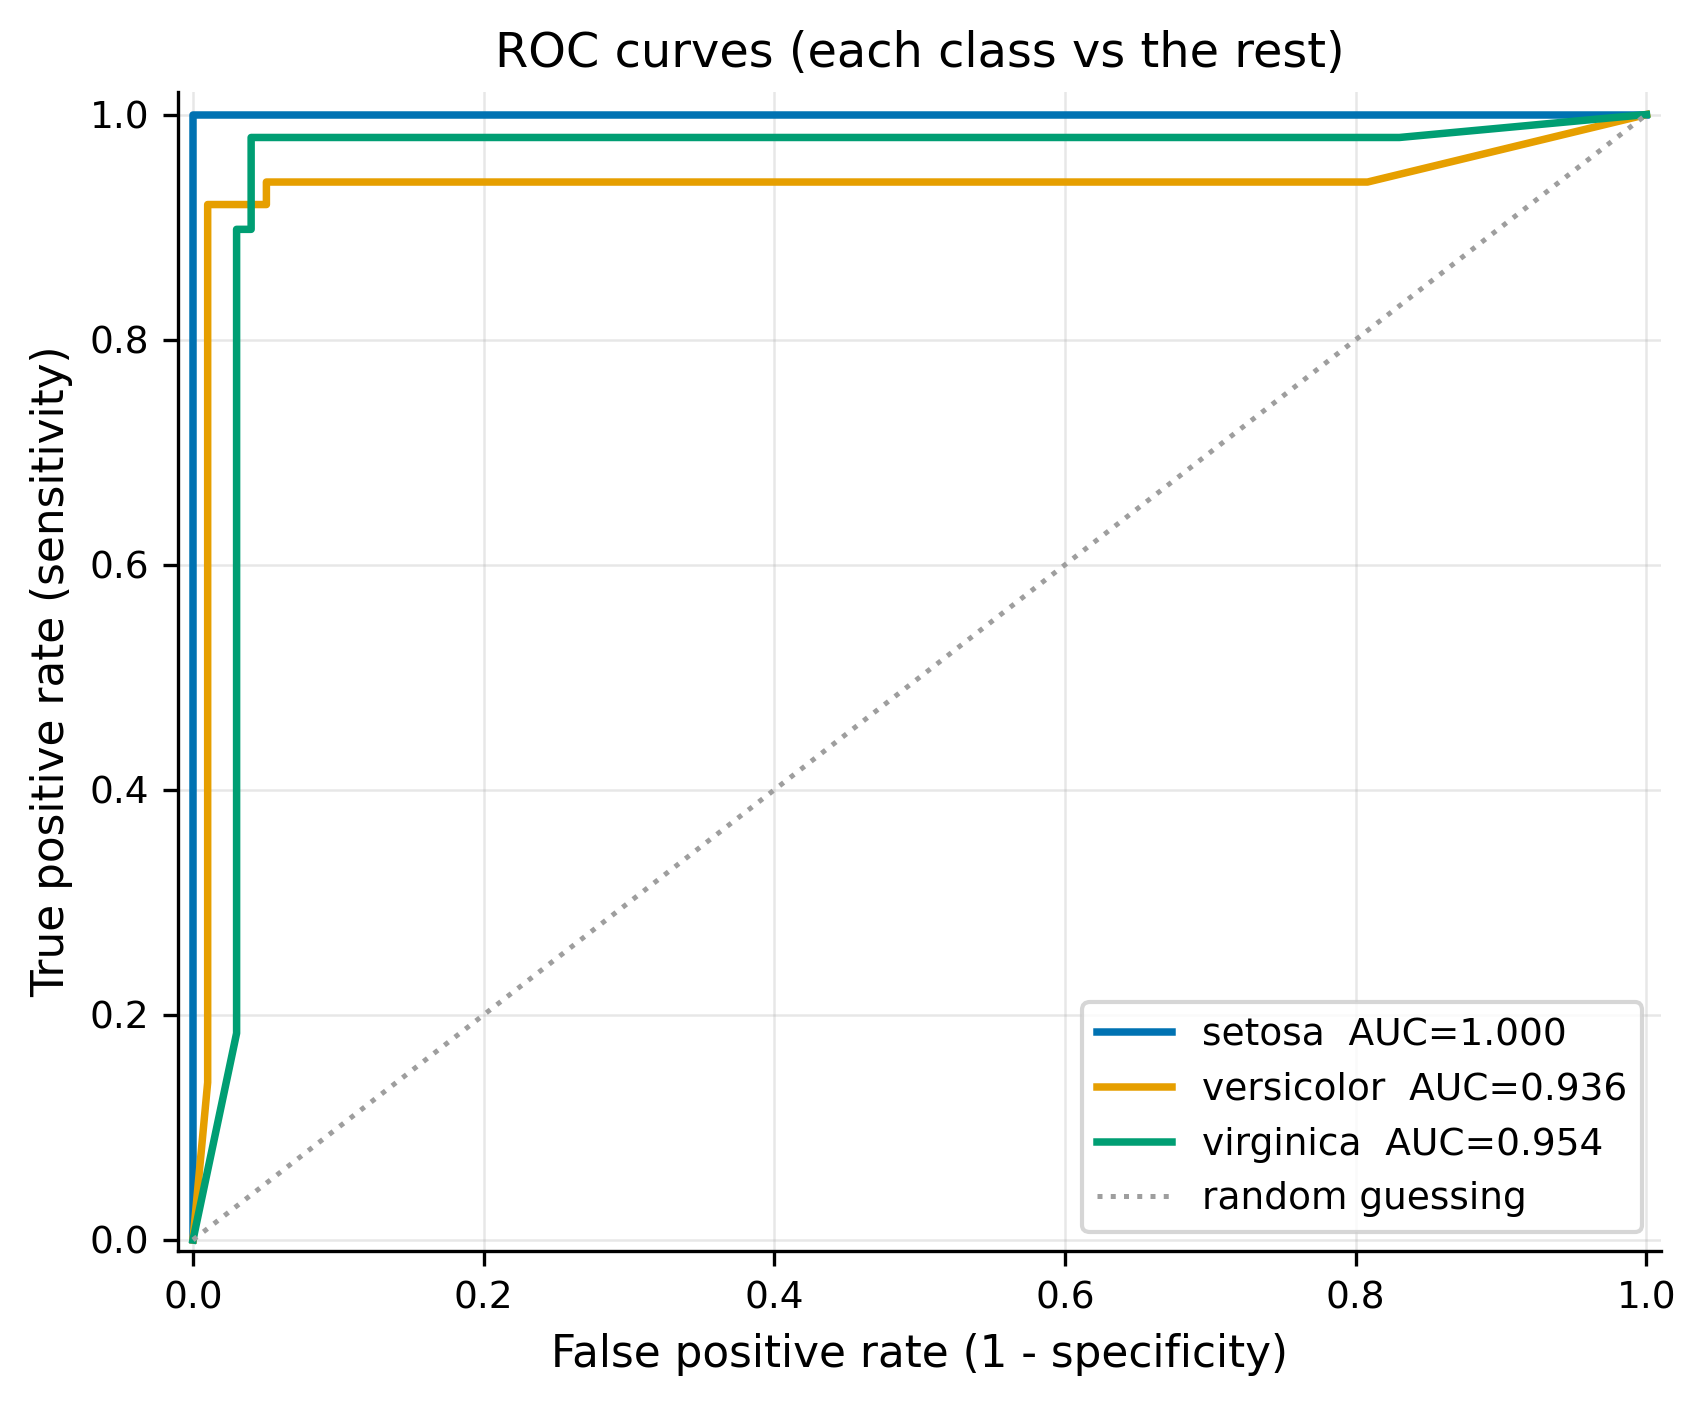
\includegraphics[width=0.62\textwidth]{figures/roc_curve.png}
\caption{ROC curve(s). The closer a curve comes to the top-left corner, the better that class is separated from the others; the dotted diagonal is random guessing. AUC summarises each curve (1 = perfect, 0.5 = random).}
\end{figure}
\subsection*{Which columns mattered}
Each column's values were shuffled, and the drop in balanced accuracy was measured on rows the model had not been trained on. A larger drop means the model relies more on that column. Values near zero (or below) mean the column did not help. Importance shows what the model uses; it does not prove cause and effect.

\begin{figure}[H]
\centering
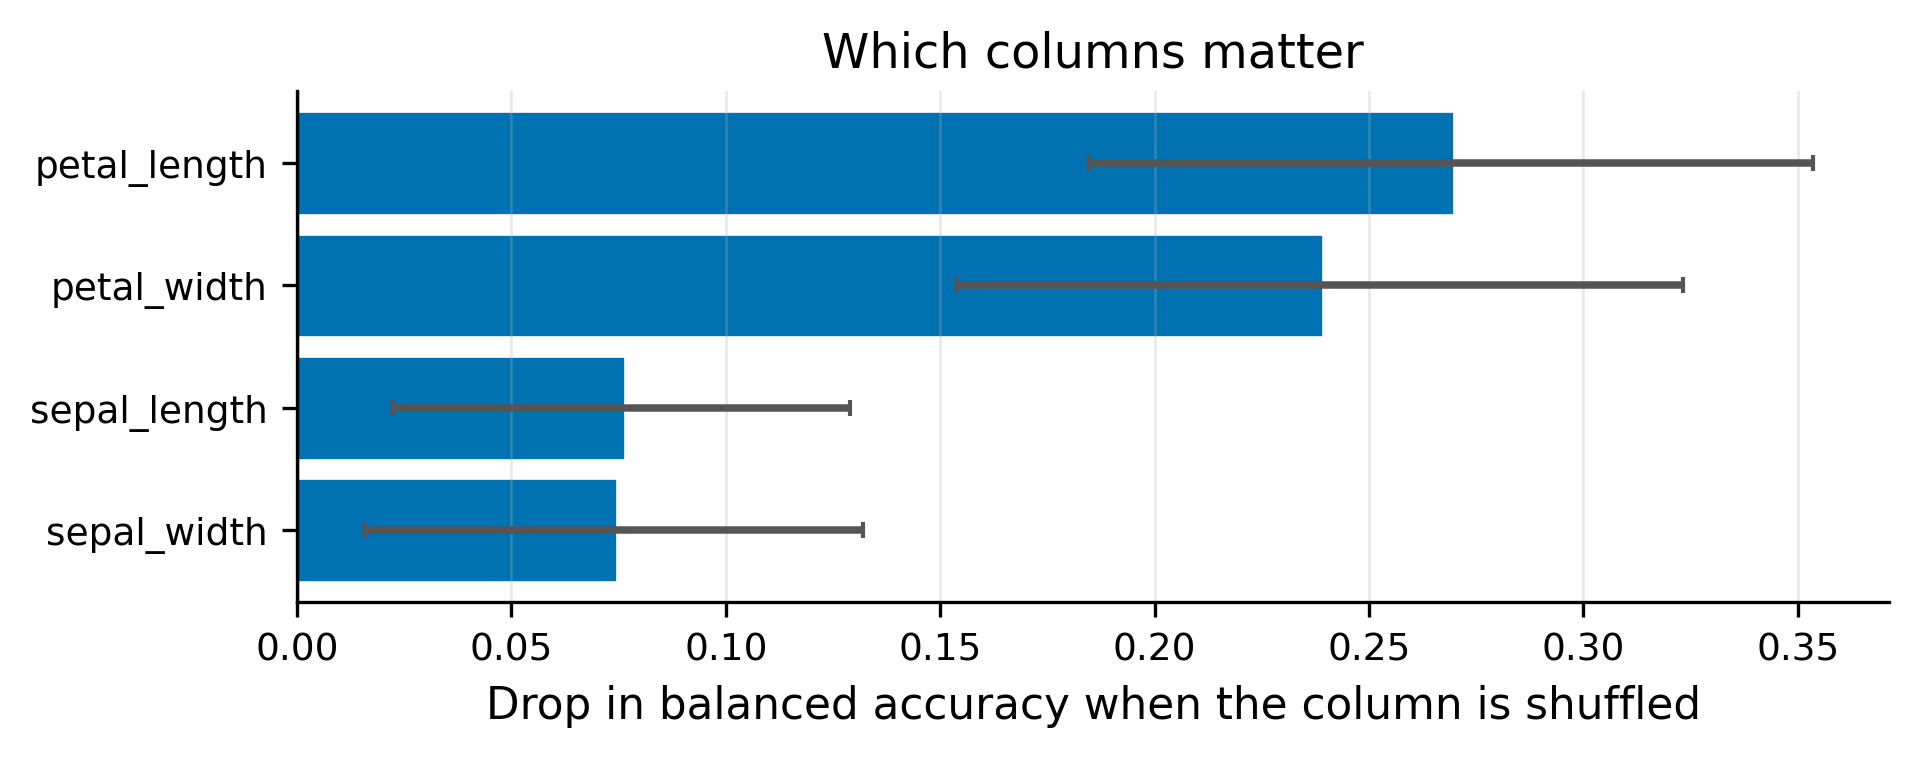
\includegraphics[width=0.72\textwidth]{figures/feature_importance.png}
\caption{Permutation importance: how much the balanced accuracy drops when a column is shuffled (mean and spread over repeated shuffles).}
\end{figure}
\begin{table}[H]
\centering
\small
\begin{tabular}{lrr}
\toprule
Column & Importance & Spread\\
\midrule
petal\_length & 0.2692 & 0.0844\\
petal\_width & 0.2385 & 0.0846\\
sepal\_length & 0.0757 & 0.0533\\
sepal\_width & 0.0739 & 0.0582\\
\bottomrule
\end{tabular}
\caption{Importance of each column.}
\end{table}
\section{Good practice when reporting}
\begin{itemize}
\item Report the final result, not the best score from the comparison table.
\item Mention the number of rows and the class sizes; results for small classes are less reliable.
\item Classifiers used default parameters (no tuning), so the results can be reproduced exactly with the same data and EasyClassifier version.
\item All choices and steps are recorded in \texttt{log.txt} in the Results folder.
\end{itemize}
\begin{thebibliography}{99}
\bibitem{easyclassifier} Hassanat, A. B. A. (2026). EasyClassifier: Machine Learning without Programming (Version 0.8.1) [Software]. Zenodo. https://doi.org/10.5281/zenodo.23122902
\bibitem{sklearn} Pedregosa, F., et al. (2011). Scikit-learn: Machine Learning in Python. Journal of Machine Learning Research, 12, 2825-2830.
\bibitem{numpy} Harris, C. R., Millman, K. J., van der Walt, S. J., et al. (2020). Array programming with NumPy. Nature, 585(7825), 357-362. https://doi.org/10.1038/s41586-020-2649-2
\bibitem{pandas} McKinney, W. (2010). Data structures for statistical computing in Python. In Proceedings of the 9th Python in Science Conference (pp. 56-61). https://doi.org/10.25080/Majora-92bf1922-00a
\bibitem{breiman1984} Breiman, L., Friedman, J. H., Olshen, R. A., \& Stone, C. J. (1984). Classification and Regression Trees. Wadsworth.
\bibitem{breiman2001} Breiman, L. (2001). Random Forests. Machine Learning, 45, 5-32. https://doi.org/10.1023/A:1010933404324
\bibitem{cortes1995} Cortes, C., \& Vapnik, V. (1995). Support-vector networks. Machine Learning, 20(3), 273-297. https://doi.org/10.1007/BF00994018
\bibitem{platt1999} Platt, J. C. (1999). Probabilistic outputs for support vector machines and comparisons to regularized likelihood methods. In A. J. Smola, P. Bartlett, B. Schölkopf, \& D. Schuurmans (Eds.), Advances in Large Margin Classifiers (pp. 61-74). MIT Press.
\bibitem{cox1958} Cox, D. R. (1958). The regression analysis of binary sequences. Journal of the Royal Statistical Society: Series B, 20(2), 215-242. https://doi.org/10.1111/j.2517-6161.1958.tb00292.x
\bibitem{cover1967} Cover, T., \& Hart, P. (1967). Nearest neighbor pattern classification. IEEE Transactions on Information Theory, 13(1), 21-27. https://doi.org/10.1109/TIT.1967.1053964
\bibitem{hand2001} Hand, D. J., \& Yu, K. (2001). Idiot's Bayes - not so stupid after all? International Statistical Review, 69(3), 385-398. https://doi.org/10.1111/j.1751-5823.2001.tb00465.x
\bibitem{rumelhart1986} Rumelhart, D. E., Hinton, G. E., \& Williams, R. J. (1986). Learning representations by back-propagating errors. Nature, 323(6088), 533-536. https://doi.org/10.1038/323533a0
\bibitem{kingma2015} Kingma, D. P., \& Ba, J. (2015). Adam: A method for stochastic optimization. In International Conference on Learning Representations (ICLR). arXiv:1412.6980.
\bibitem{hassanat2022} Hassanat, A. B., Alkafaween, E., Tarawneh, A. S., \& Elmougy, S. (2022). Applications review of Hassanat distance metric. In 2022 International Conference on Emerging Trends in Computing and Engineering Applications (ETCEA), Karak, Jordan (pp. 1-6). IEEE. https://doi.org/10.1109/ETCEA57049.2022.10009844
\bibitem{hassanat2014} Hassanat, A. B. (2014). Dimensionality invariant similarity measure. arXiv preprint arXiv:1409.0923. https://arxiv.org/abs/1409.0923
\bibitem{kohavi1995} Kohavi, R. (1995). A study of cross-validation and bootstrap for accuracy estimation and model selection. In Proceedings of the 14th International Joint Conference on Artificial Intelligence (IJCAI) (pp. 1137-1143).
\bibitem{varma2006} Varma, S., \& Simon, R. (2006). Bias in error estimation when using cross-validation for model selection. BMC Bioinformatics, 7, 91. https://doi.org/10.1186/1471-2105-7-91
\bibitem{cawley2010} Cawley, G. C., \& Talbot, N. L. C. (2010). On over-fitting in model selection and subsequent selection bias in performance evaluation. Journal of Machine Learning Research, 11, 2079-2107.
\bibitem{brodersen2010} Brodersen, K. H., Ong, C. S., Stephan, K. E., \& Buhmann, J. M. (2010). The balanced accuracy and its posterior distribution. In 20th International Conference on Pattern Recognition (pp. 3121-3124). IEEE. https://doi.org/10.1109/ICPR.2010.764
\bibitem{fawcett2006} Fawcett, T. (2006). An introduction to ROC analysis. Pattern Recognition Letters, 27(8), 861-874. https://doi.org/10.1016/j.patrec.2005.10.010
\bibitem{matplotlib} Hunter, J. D. (2007). Matplotlib: A 2D graphics environment. Computing in Science \& Engineering, 9(3), 90-95. https://doi.org/10.1109/MCSE.2007.55
\end{thebibliography}
\end{document}
